% Created 2024-10-16 śro 21:35
% Intended LaTeX compiler: pdflatex
\documentclass[../main.tex]{subfiles}

% \usepackage[a4paper, margin=3cm]{geometry}
% \usepackage{amssymb} // not working

\usepackage[T1]{fontenc}
\usepackage[utf8]{inputenc}
\usepackage{graphicx}
\usepackage{longtable}
\usepackage{wrapfig}
\usepackage{rotating}
\usepackage[normalem]{ulem}
\usepackage{amsmath}
\usepackage{capt-of}
\usepackage{hyperref}
\usepackage{siunitx}
\usepackage{float}
\usepackage[polish]{babel}

\graphicspath{{../}}
\author{Wojciech Paderewski}
\date{\today}
\title{Koncepcja ukladu}
\hypersetup{
 pdfauthor={Wojciech Paderewski},
 pdftitle={Koncepcja ukladu},
 pdfkeywords={},
 pdfsubject={},
 pdflang={Polish}}

 
 \begin{document}
 Etap koncepcyjny został podzielony na dwa etapy: koncepcję układu oraz realizacje. W tym rozdziale znajduje się ogólna koncepcja 
 działania układu, która nie jest związana z konkretnymi elementami sprzętowymi, a jedynie z funkcjonalnościami, które mają być zrealizowane.
 \subsection{Założenia projektowe}
Zgodnie z celem pracy, określono następujące założenia projektowe:
\begin{itemize}
    \item Funkcjonalność ustawiania godziny budzika bedzie realizowana przez zewnętrzny serwer dla wygody użytkownika, który nie musi dostosowywać czasu ręcznie.
    \item Na wyświetlaczu Nixie będą wyświetlane godziny, minuty, sekundy.
    \item Od spodu obudowy będą umieszczone paski LED, które będą podświetlały obudowę i będą wyświetlane animacje podczas alarmu.
    \item Alarm będzie sygnalizowany dźwiękiem oraz miganiem pasków LED.
    \item Dźwięk może być odtwarzany z głośnika wbudowanego w obudowę lub z zewnętrznego głośnika komunikującego się z serwerem przez Wi-Fi.
    \item Wyłączanie alarmu będzie możliwe poprzez przycisk na obudowie, aplikację mobilną lub zewnętrzny przycisk połączony z serwerem.
    \item W przypadku braku połączenia z serwerem, czas będzie mierzony przez RTC wbudowany w mikrokontroler.
    \item Programowa oraz manualna regulacja jasności wyświetlacza Nixie oraz pasków LED.
\end{itemize}
Powyższe założenia powodują podzielnie projektu na poszczególne moduły realizujące poszczególne funkcje, które będą opisane w dalszej części dokumentu.
Ogólna koncepcja układu jest przedstawiona na rysunku \ref{fig:concept}.
\begin{figure}[H]
    \centering
    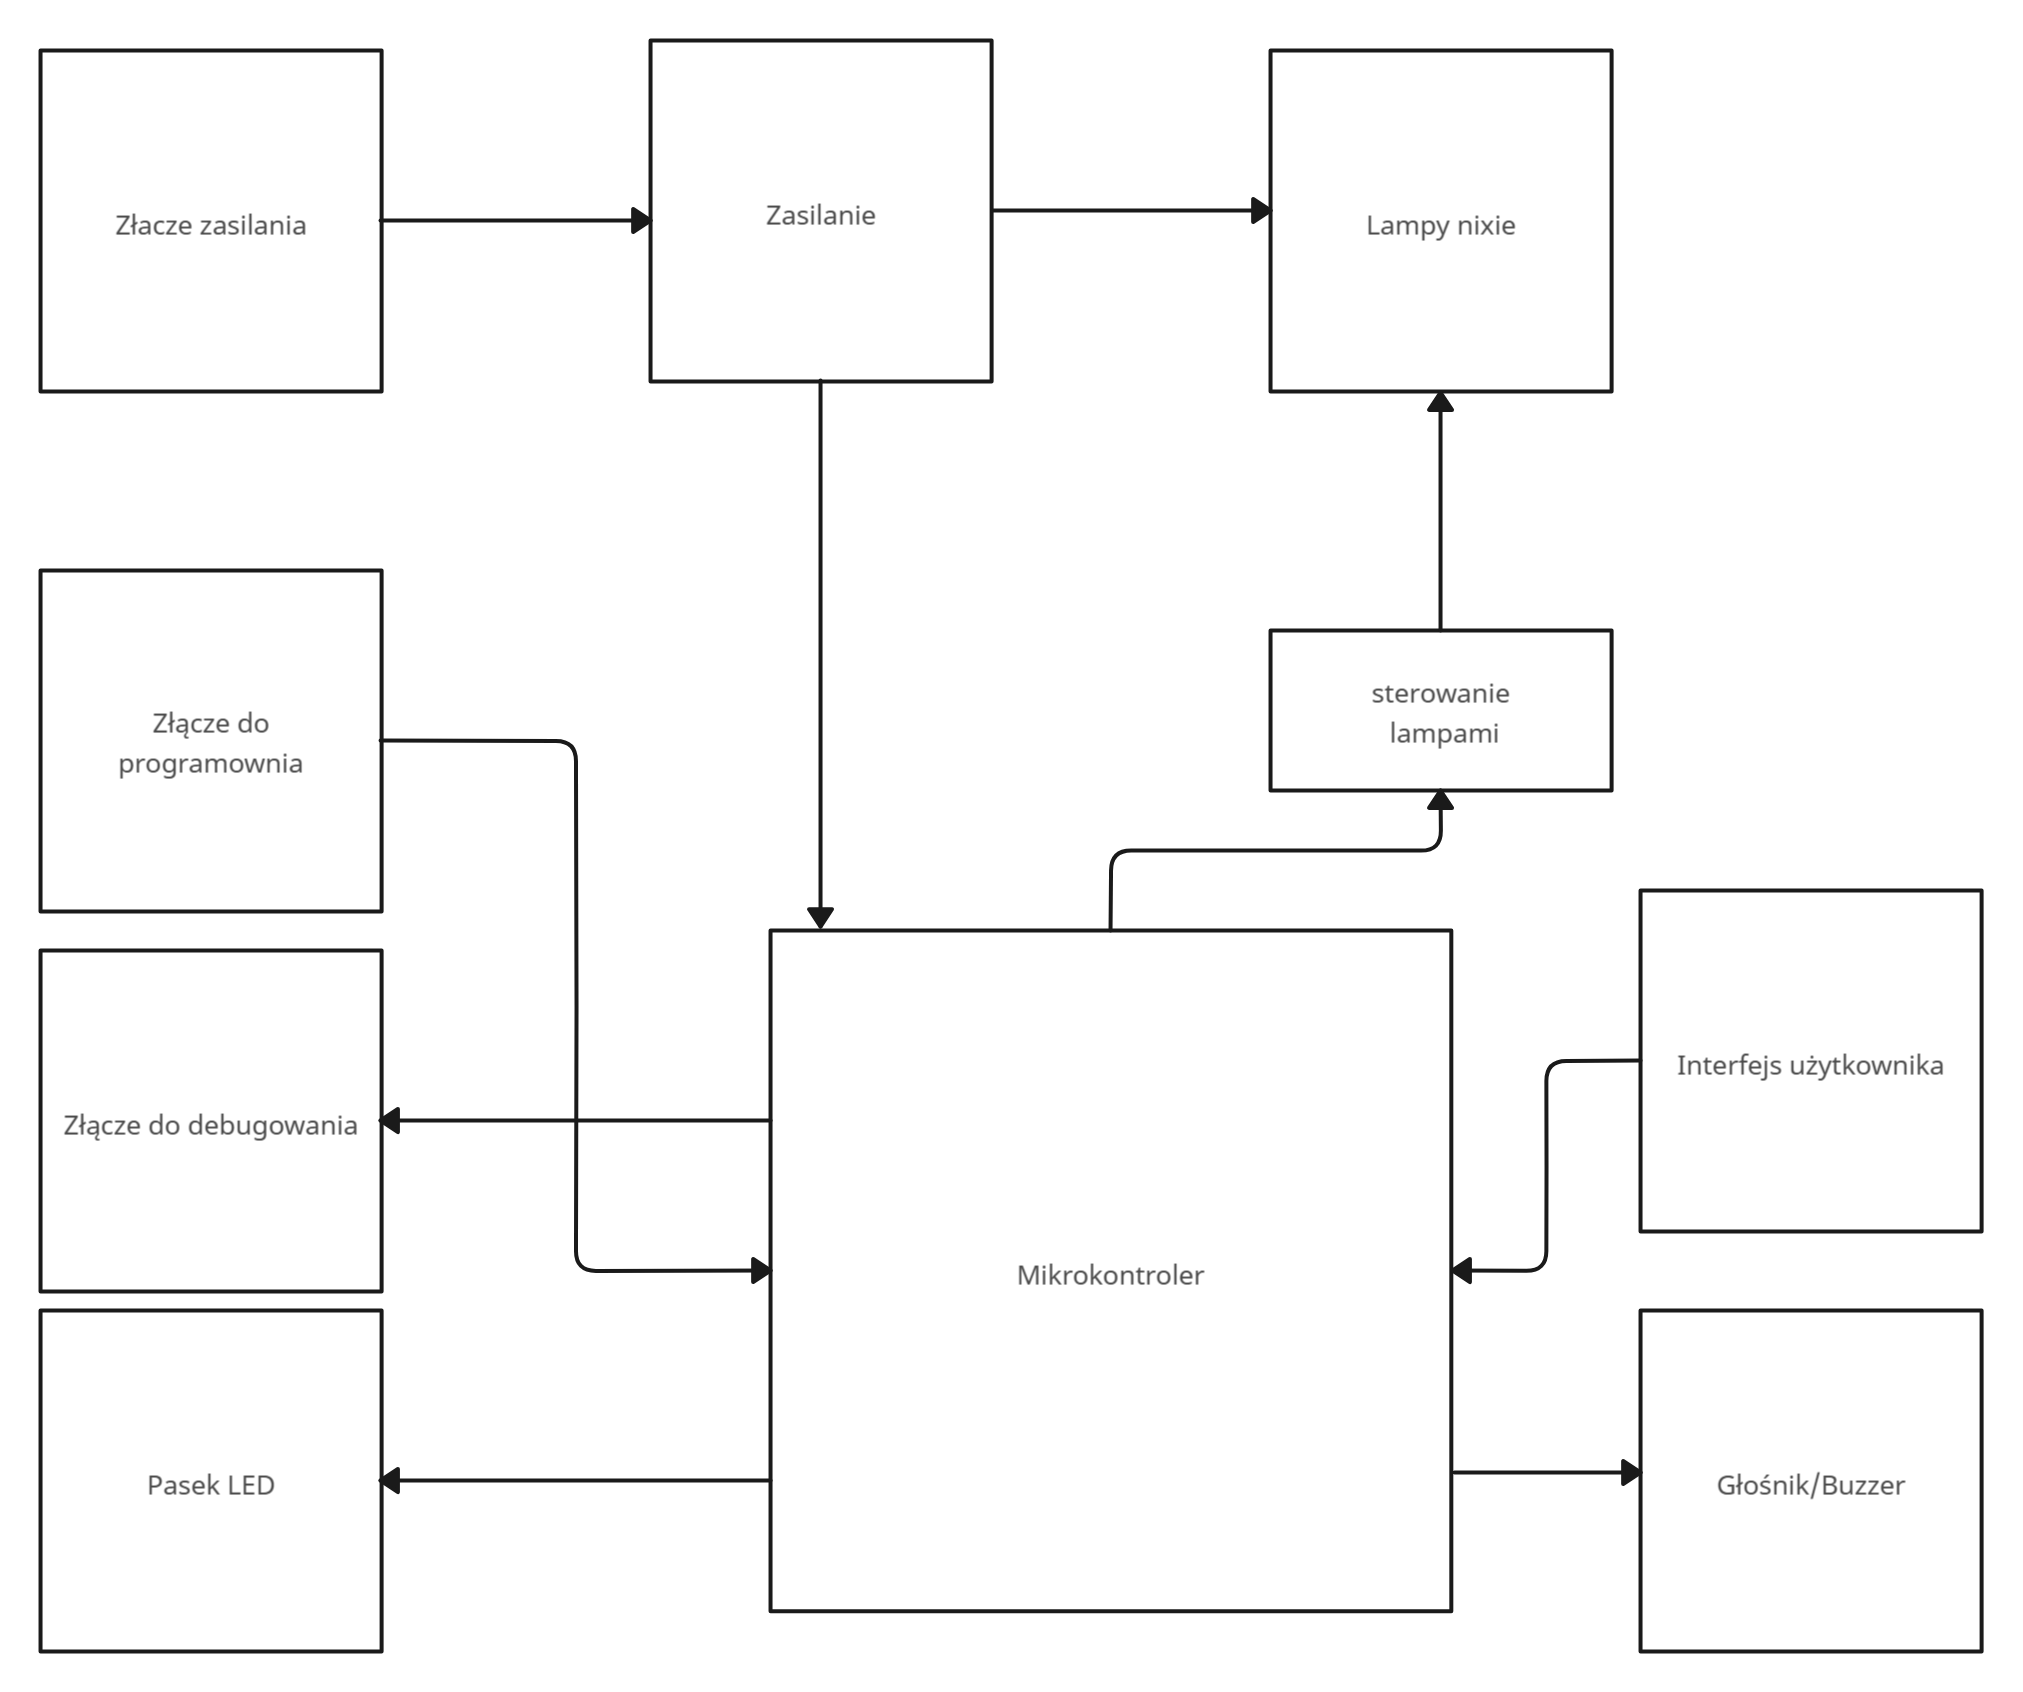
\includegraphics[width=0.55\textwidth]{Nixie-concept.png}
    \caption{Ogólna koncepcja układu}
    \label{fig:concept}
\end{figure}
Sekcja opisana jako \textit{zasilanie} będzie odpowiedzialna za zasilanie wszystkich elementów układu, w tym lamp Nixie, pasków LED, mikrokontrolera oraz głośnika,
więc będzie wymagane rozbicie jej na kilka podsekcji, ponieważ będą potrzebne różne napięcia. Lampy Nixie potrzebują zasilania wysokim napięciem,
natomiast pozostałe elementy potrzebują zdecydowanie niższych napięć. Blok \textit{sterowanie lampami Nixie} będzie odpowiedzialny za wyświetlanie odpowiednich cyfr na lampach.
Sekcja \textit{Interfejs użytkownika} będzie odpowiedzialna za interakcję z użytkownikiem, w tym regulacja jasności oraz wyłączania alarmu ,ważne by interfejs był 
intuicyjny i jak najbardziej rozwojowy na potencjalne przyszłe funkcje.
\subsection{Ogólny schemat komunikacji z serwerem}
Urządzenie będzie musiało komunikować się z serwerem czasu, który będzie dostarczał aktualny czas, a także z serwerem Home Assistant, który będzie interfejsem użytkownika.
Komunikacja z serwerem czasu będzie odbywała się poprzez protokół NTP, ponieważ jest to najbardziej optymalne rozwiązanie, ponieważ inne protokoły opisane w rozdziale \ref{sec:serwery_czasu}
służą do zapewnienia większej dokładności czasu, co nie jest wymagane w tym projekcie. Inne protokoły wymagają też większej ilości zasobów lub specjalistycznego sprzętu.
Kolejną zaletą wyboru NTP jest to, że jest to najbardziej popularny protokół do synchronizacji czasu w sieciach komputerowych, co sprawia, że jest on najbardziej przetestowany i stabilny.
Posiada on wiele implementacji, które są dostępne na wielu platformach, w tym na platformę ESP32.
Komunikacja z serwerem Home Assistant będzie odbywała się poprzez protokół MQTT, który jest bardzo popularnym protokołem w IoT, co pozwoli na łatwe rozbudowanie funkcjonalności.
Połączenia te przedstawione są na rysunku \ref{fig:communication}.
\begin{figure}[H]
    \centering
    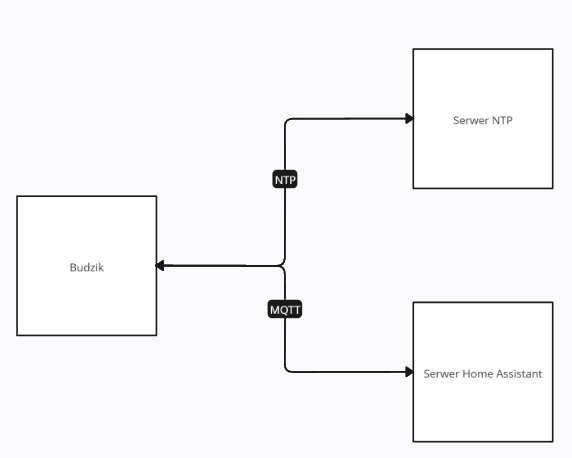
\includegraphics[width=0.8\textwidth]{polaczenia.png}
    \caption{Ogólny schemat komunikacji z serwerem}
    \label{fig:communication}
\end{figure}

\end{document}
